\documentclass[xcolor=pdftex,romanian,colorlinks]{beamer}

\usepackage[export]{adjustbox}
\usepackage{../tslides}
\usepackage[all]{xy}
\usepackage{pgfplots}
\usepackage{flowchart}
\usetikzlibrary{arrows,positioning,calc}
\lstset{language=Haskell}
\lstset{escapeinside={(*@}{@*)}}

\AtBeginSection[]{
  \begin{frame}
  \vfill
  \centering
  \begin{beamercolorbox}[sep=8pt,center,shadow=true,rounded=true]{title}
    \usebeamerfont{title}\insertsectionhead\par%
  \end{beamercolorbox}
  \vfill
  \end{frame}
}


\title[PD---Intrare/Ieșire]{Programare declarativă\thanks{bazat pe cursul \emph{Informatics 1: Functional Programming} de la \emph{University of Edinburgh}}}

\subtitle{Intrare/Ieșire}

\begin{document}
\begin{frame}
  \titlepage
\end{frame}

\section{Despre utilitate și siguranță}

\begin{frame}{Simon Peyton Jones --- Haskell is Useless}{\url{http://www.youtube.com/watch?v=iSmkqocn0oQ}}
\end{frame}

\section{Despre intenție și acțiune}

\begin{frame}{Mind-Body Problem --- Comandă vs. Execuție}{Care e legătura dintre intenție și acțiune, dintre percepție și înțelegere?}

\begin{minipage}{.4\columnwidth}
\begin{itemize}
\item Idealism (Platon)
\item Dualism (Descartes)
\item Fizicalism (materialism)
\item Neutral Monism
\end{itemize}
\end{minipage}
\begin{minipage}{.45\columnwidth}
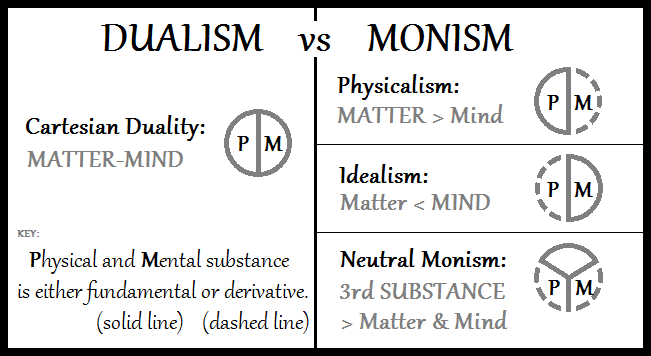
\includegraphics[scale=.4]{Dualism-vs-Monism.png}
\end{minipage}
\end{frame}

\section{Comenzi în Haskell}

\begin{frame}[fragile]{Afișează un caracter!}
\begin{asciihs}
   putChar :: Char -> IO ()
\end{asciihs}
\begin{block}{Exemplu}
\begin{asciihs}
   putChar '!'
\end{asciihs}
rerpezintă o comandă care, \alert{dacă va fi executată}, va afișa un semn de exclamare.
\end{block}

\end{frame}

\begin{frame}[fragile]{Combină două comenzi!}
\begin{asciihs}
   (>>) :: IO () -> IO () -> IO ()
   putChar :: Char -> IO ()
\end{asciihs}
\begin{block}{Exemplu}
\begin{asciihs}
      putChar '?' >> putChar '!'
\end{asciihs}
rerpezintă o comandă care, \alert{dacă va fi executată}, va afișa un semn de întrebare urmat de un semn de exclamare .
\end{block}
\end{frame}

\begin{frame}[fragile]{Stai locului! (nu face nimic!)}
\begin{asciihs}
   done :: IO ()
\end{asciihs}

\lstinline$done$ rerpezintă o comandă care, \alert{dacă va fi executată}, nu va face nimic.
\end{frame}

\subsection{Funcții folosind comenzi}

\begin{frame}[fragile]{Afișează un șir de caractere}
\begin{asciihs}
   putStr :: String -> IO ()
   putStr []     = done
   putStr (x:xs) = putChar x >> putStr xs
\end{asciihs}

\begin{block}{Exemplu}
\begin{asciihs}
      putStr "?!" == putChar '?' >> (putChar '!' >> done)
\end{asciihs}
rerpezintă o comandă care, \alert{dacă va fi executată}, va afișa un semn de întrebare urmat de un semn de exclamare.
\end{block}
\end{frame}

\begin{frame}[fragile]{\lstinline$putStr$ folosind funcționale}
\begin{asciihs}
   putStr     :: String -> IO ()
   putStr     = foldr (>>) done . map putChar
\end{asciihs}
\end{frame}

\begin{frame}[fragile]{\lstinline$(IO(), (>>), done)$ e monoid}
\begin{asciihs}
   m >> done           =   m
   done >> m           =   m
   (m >> n) >> o       =   m >> (n >> o)
\end{asciihs}
\end{frame}

\begin{frame}[fragile]{Și totuși, când sunt executate comenzile?}{\lstinline$main$}

\begin{block}
{Fișierul PutStr.hs}
\begin{asciihs}
   module PutStr where
   
   main :: IO ()
   main = putStr "?!"
\end{asciihs}
\end{block}

Rularea programului are ca \structure{efect} executarea comenzii specificate de \lstinline$main$:
\begin{asciihs}
   08-io$ runghc PutStr.hs
   ?!08-io$
\end{asciihs}
\end{frame}

%Main
%By now you may be desperate to know how is a command ever performed? Here
%is the file Confused.hs:
%   module Confused where
%
%
%Running this program prints an indicator of perplexity:
%   [melchior]dts: runghc Confused.hs
%   ?![melchior]dts:
%
%Thus main is the link from Haskell’s mind to Haskell’s body — the analogue of
%Descartes’s pineal gland.
\begin{frame}[fragile]{Afișează și treci pe rândul următor}
\begin{asciihs}
   putStrLn :: String -> IO ()
   putStrLn xs = putStr xs >> putChar '\n'
\end{asciihs}

\begin{block}
{Fișierul ScrieLinie.hs}
\begin{asciihs}
   module ScrieLinie where
   
   start :: IO ()
   start = putStrLn "?!"
\end{asciihs}
\end{block}


Rulare cu compilare:
\begin{asciihs}
08-io$ ghc ScrieLinie.hs -main-is ScrieLinie.start -o scrie
[1 of 1] Compiling ScrieLinie  (ScrieLinie.hs, ScrieLinie.o)
Linking scrie ...
08-io$ ./scrie
?!
08-io$
\end{asciihs}

\end{frame}


\section{Validitatea raționamentelor}

%$
\begin{frame}[fragile]{Raționamentele substitutive își pierd valabilitatea}
{În limbaje cu efecte laterale}


\begin{block}
{Program 1}
\begin{asciic}
int main() { cout << "HA!"; cout << "HA!"; }
\end{asciic}
\end{block}

\begin{block}
{Program 2}
\begin{asciic}
void dup(auto& x) { x ; x; }
int main() { dup(cout << "HA!"); }
\end{asciic}
\end{block}

\begin{block}
{Program 3}
\begin{asciic}
void dup(auto x) { x() ; x(); }
int main() { dup( []() { cout << "HA!"; } ); }
\end{asciic}
\end{block}

\end{frame}

\begin{frame}[fragile]{Raționamentele substitutive sunt valabile}
{În Haskell}
\begin{block}{Expresii}
\begin{asciihs}
   (1+2) * (1+2)
\end{asciihs}
este echivalentă cu expresia
\begin{asciihs}
   let x = 1+2 in x * x
\end{asciihs}
și se evaluează amândouă la 9
\end{block}

\begin{block}{Comenzi}
\begin{asciihs}
   putStr "HA!" >> putStr "HA!"
\end{asciihs}
este echivalentă cu
\begin{asciihs}
   let m = putStr "HA!" in m >> m
\end{asciihs}
si amândouă afișează "HA!HA!".
\end{block}
\end{frame}

\section{Comenzi cu valori}

\begin{frame}[fragile]{Comenzi cu valori}
\begin{itemize}
\item \lstinline$IO ()$ corespunde comenzilor care nu produc rezultate
\begin{itemize}
\item \lstinline$()$ este tipul unitate care conține doar valoarea \lstinline$()$
\end{itemize}
\vitem În general, \structure{\lstinline$IO a$}  corespunde comenzilor care produc rezultate de tip \structure{\lstinline$a$}.
\begin{itemize}
\item \lstinline$IO Char$ corespunde comenzilor care produc rezultate de tip \lstinline$Char$
\end{itemize}
\end{itemize}
\end{frame}


\begin{frame}[fragile]{Citește un caracter!}
\begin{asciihs}
   getChar :: IO Char
\end{asciihs}

\begin{itemize}
\item Dacă „șirul de intrare” conține \lstinline$"abc"$
\item atunci \lstinline$getChar$ produce:
\begin{itemize}
\item \lstinline$'a'$ 
\item șirul rămas de intrare \lstinline$"bc"$
\end{itemize}
\end{itemize}
\end{frame}


\begin{frame}[fragile]{Produ o valoare făra să faci nimic!}{Din pălărie}
\begin{asciihs}
   return :: a -> IO a
\end{asciihs}

Asemănatoar cu \lstinline$done$, nu face nimic, dar produce o valoare.
\begin{block}{Exemplu}
\begin{asciihs}
   return ""
\end{asciihs}
\begin{itemize}
\item Dacă „șirul de intrare” conține \lstinline$"abc"$
\item atunci \lstinline$return ""$ produce:
\begin{itemize}
\item valoarea \lstinline$""$ 
\item șirul (neschimbat) de intrare \lstinline$"abc"$
\end{itemize}
\end{itemize}
\end{block}
\end{frame}


\begin{frame}[fragile]{Combinarea comenzilor cu valori}
{Operatorul de legare / bind}
\begin{asciihs}
   (>>=) :: IO a -> (a -> IO b) -> IO b
\end{asciihs}
\begin{block}{Exemplu}
\begin{asciihs}
   getChar >>= \x -> putChar (toUpper x)
\end{asciihs}
\begin{itemize}
\item Dacă „șirul de intrare” conține \lstinline$"abc"$
\item atunci comanda de mai sus, atunci când se execută, produce:
\begin{itemize}
\item ieșirea "A"
\item șirul rămas de intrare \lstinline$"bc"$
\end{itemize}
\end{itemize}
\end{block}
\end{frame}

\begin{frame}[fragile]{Operatorul de legare / bind}{Mai multe detalii}
\begin{asciihs}
     (>>=) :: IO a -> (a -> IO b) -> IO b
\end{asciihs}

\begin{itemize}
\item Dacă fiind o comandă care produce o valoare de tip a

\lstinline$m :: IO a$
\item Data fiind o funcție care pentru o valoare de tip a se evaluează la o comandă de tip b

\lstinline$k :: a -> IO b$
\item Atunci 

\lstinline$m >>= k :: IO b$

este comanda care, dacă se va executa:
\begin{itemize}
\item Mai întâi efectuează m, obținând valoarea x de tip a
\item Apoi efectuează comanda k x obținând o valoare y de tip b
\item Produce y ca rezultat al comenzii
\end{itemize}
\end{itemize}
\end{frame}

\begin{frame}[fragile]{Citește o linie!}
\begin{asciihs}
   getLine :: IO String
   getLine = getChar >>= \x ->
              if x == '\n' then
                return []
              else
                getLine >>= \xs ->
                return (x:xs)
\end{asciihs}

\begin{block}
{Exemplu}
Dat fiind șirul de intrare \lstinline$"abc\ndef"$, getLine produce șirul "abc" și șirul rămas de intrare e "def"
\end{block}
\end{frame}

\begin{frame}[fragile]{Comenzile sunt cazuri speciale de comenzi cu valori}
\begin{block}{done e caz special de return}
\begin{asciihs}
   done      :: IO ()
   done      = return ()
\end{asciihs}
\end{block}
\begin{block}{\lstinline$>>$ e caz special de \lstinline$>>=$ }
\begin{asciihs}
   (>>)      :: IO () -> IO () -> IO ()
   m >> n    = m >>= \ () -> n
\end{asciihs}
\end{block}
\end{frame}

\begin{frame}[fragile]{Operatorul de legare e similar cu \lstinline$let$}
\begin{block}
{Operatorul \lstinline$let$} 
\begin{asciihs}
    let x = m in n  
\end{asciihs}
\end{block}

\begin{block}
{\lstinline$let$ ca aplicație de funcții} 
\begin{asciihs}
    (\ x -> n) m
\end{asciihs}
\end{block}

\begin{block}
{Operatorul de legare} 
\begin{asciihs}
    m >>= \ x -> n 
\end{asciihs}
\end{block}

\end{frame}
%An analogue of “let”
%Although it may seem odd at first sight, this combinator is reassuringly similar to
%the familiar Haskell “let” expression. Here is a type rule for “let”.
%
%                        E ` m :: a
%                        E, x :: a ` n :: b
%                        E ` let x = m in n :: b
%
%Typically, “bind” is combined with lambda expressions in a way that resembles
%“let” expressions. Here is the corresponding type rule.
%
%                       E ` m :: IO a
%                       E, x :: a ` n :: IO b
%                       E ` m >>= \x -> n :: IO b
\begin{frame}[fragile]{}
\begin{asciihs}
\end{asciihs}
\end{frame}
%
%This program echoes its input to its output, putting everything in upper case, until
%an empty line is entered.
\begin{frame}[fragile]{De la intrare la ieșire}
\begin{asciihs}
   echo :: IO ()
   echo = getLine >>= \line ->
           if line == "" then
             return ()
           else
             putStrLn (map toUpper line) >>
             echo

   main :: IO ()
   main = echo
\end{asciihs}
\onslide<2>
\begin{block}{Test}
\begin{asciihs}
$ runghc Echo.hs
One line
ONE LINE
And, another line!
AND, ANOTHER LINE!
\end{asciihs}
\end{block}

\end{frame}
%$
%  [melchior]dts:
%    Part V
%
\section{Notația do}
\begin{frame}[fragile]{Citirea unei linii în notație „do”}
\vspace{-1ex}
\begin{asciihs}
   getLine :: IO String
   getLine = getChar >>= \x ->
              if x == '\n' then
                return []
              else
                getLine >>= \xs ->
                return (x:xs)
\end{asciihs}
\vspace{-1ex}
Echivalent cu:
\begin{asciihs}
   getLine :: IO String
   getLine = do {
                x <- getChar;
                if x == '\n' then
                  return []
                else do {
                  xs <- getLine;
                  return (x:xs)
                }
              }
\end{asciihs}

\end{frame}
%
%
%is equivalent to
\begin{frame}[fragile]{Echo în notația „do”}
\vspace{-1ex}
\begin{asciihs}
   echo :: IO ()
   echo = getLine >>= \line ->
           if line == "" then
             return ()
           else
             putStrLn (map toUpper line) >>
             echo

\end{asciihs}
\vspace{-1ex}
Echivalent cu
\begin{asciihs}
   echo :: IO ()
   echo = do {
             line <- getLine;
             if line == "" then
               return ()
             else do {
               putStrLn (map toUpper line);
               echo
             }
           }
\end{asciihs}
\end{frame}

\begin{frame}[fragile]{Notația „do” în general}
\begin{itemize}
\item Fiecare linie \lstinline$x <- e; ...$ devine \lstinline$e >>= \x -> ...$
\item Fiecare linie \lstinline$e; ...$ devine \lstinline$e >> ...$
\end{itemize}
De exemplu
\begin{asciihs}
   do { x1 <- e1;
        x2 <- e2;
        e3;
        x4 <- e4;
        e5;
        e6 }
\end{asciihs}
e echivalent cu
\begin{asciihs}
   e1   >>= \x1 ->
   e2   >>= \x2 ->
   e3   >>
   e4   >>= \x4 ->
   e5   >>
   e6
\end{asciihs}
\end{frame}


%“Do” notation in general
%For example,
%
%is equivalent to
%Part VI
%
%Monads
%Monoids
%A monoid is a pair of an operator (@@) and a value u, where the operator has the
%value as identity and is associative.
%   u @@ x              =   x
%   x @@ u              =   x
%   (x @@ y) @@ z       =   x @@ (y @@ z)
%
%Examples of monoids:
%
%
%                                 (+) and 0
%                                 (*) and 1
%                               (||) and False
%                               (&&) and True
%                                (++) and []
%                               (>>) and done
%Monads
%We know that (>>) and done satisfy the laws of a monoid.
%   done >> m          =   m
%   m >> done          =   m
%   (m >> n) >> o      =   m >> (n >> o)
%
%Similarly, (>>=) and return satisfy the laws of a monad.
%   return v >>= \x -> m               =   m[x:=v]
%   m >>= \x -> return x               =   m
%   (m >>= \x -> n) >>= \y-> o         =   m >>= \x -> (n >>= \y -> o)
%Laws of Let
%We know that (>>) and done satisfy the laws of a monoid.
%   done >> m           =   m
%   m >> done           =   m
%   (m >> n) >> o       =   m >> (n >> o)
%
%Similarly, (>>=) and return satisfy the laws of a monad.
%   return v >>= \x -> m                 =   m[x:=v]
%   m >>= \x -> return x                 =   m
%   (m >>= \x -> n) >>= \y-> o           =   m >>= \x -> (n >>= \y -> o)
%
%The three monad laws have analogues in “let” notation.
%   let x = v in m   =   m[x:=v]
%   let x = m in x   =   m
%   let y = (let x = m in n) in o
%                    =   let x = m in (let y = n in o)
%“Let” in languages with and without effects
%   let x = v in m   =   m[x:=v]
%   let x = m in x   =   m
%   let y = (let x = m in n) in o
%                    =   let x = m in (let y = n in o)
%
%These laws hold even in languages with side effects. For the first law to be true, v
%must be not an arbitrary term but a value, such as a constant or a variable (but not
%a function application). A value immediately evaluates to itself, hence it can have
%no side effects.
%While in such languages one only has the above three laws for “let”, in Haskell
%one has a much stronger law, where one may replace a variable by any term, rather
%than by any value.
%   let x = n in m         =   m[x:=n]
%        Part VII
%
%Roll your own monad—IO
%The Monad type class
%  class Monad m where
%    return :: a -> m a
%    (>>=) :: m a -> (a -> m b) -> m b
%My own IO monad (1)
%   module MyIO(MyIO, myPutChar, myGetChar, convert) where
%
%   type Input = String
%   type Remainder = String
%   type Output = String
%
%   data MyIO a     =   MyIO (Input -> (a, Remainder, Output))
%
%   apply :: MyIO a -> Input -> (a, Remainder, Output)
%   apply (MyIO f) inp = f inp
%
%Note that the type MyIO is abstract. The only operations on it are the monad
%operations, myPutChar, myGetChar, and convert. The operation apply is
%not exported from the module.
%My own IO monad (2)
%   myPutChar :: Char -> MyIO ()
%   myPutChar c = MyIO (\inp -> ((), inp, [c]))
%
%   myGetChar :: MyIO Char
%   myGetChar = MyIO (\(ch:rem) -> (ch, rem, ""))
%
%For example,
%   apply   myGetChar "abc" == (’a’,    "bc", "")
%   apply   myGetChar "bc"   == (’b’,   "c", "")
%   apply   (myPutChar ’A’) "def" ==    ((), "def", "A")
%   apply   (myPutChar ’B’) "def" ==    ((), "def", "B")
%My own IO monad (3)
%   instance Monad MyIO where
%     return x = MyIO (\inp -> (x, inp, ""))
%     m >>= k   = MyIO (\inp ->
%                    let (x, rem1, out1) = apply m inp in
%                    let (y, rem2, out2) = apply (k x) rem1 in
%                    (y, rem2, out1++out2))
%
%For example
%   apply
%     (myGetChar >>= \x -> myGetChar >>= \y -> return [x,y])
%     "abc"
%   == ("ab", "c", "")
%   apply
%     (myPutChar ’A’ >> myPutChar ’B’)
%     "def"
%   == ((), "def", "AB")
%   apply
%     (myGetChar >>= \x -> myPutChar (toUpper x))
%     "abc"
%   == ((), "bc", "A")
%My own IO monad (4)
%   convert :: MyIO () -> IO ()
%   convert m = interact (\inp ->
%                   let (x, rem, out) = apply m inp in
%                   out)
%
%Here
%   interact :: (String -> String) -> IO ()
%
%is part of the standard prelude. The entire input is converted to a string (lazily) and
%passed to the function, and the result from the function is printed as output (also
%lazily).
%Using my own IO monad (1)
%  module MyEcho where
%
%  import Char
%  import MyIO
%
%  myPutStr :: String -> MyIO ()
%  myPutStr = foldr (>>) (return ()) . map myPutChar
%
%  myPutStrLn :: String -> MyIO ()
%  myPutStrLn s = myPutStr s >> myPutChar ’\n’
%Using my own IO monad (2)
%  myGetLine :: MyIO String
%  myGetLine = myGetChar >>= \x ->
%               if x == ’\n’ then
%                 return []
%               else
%                 myGetLine >>= \xs ->
%                 return (x:xs)
%
%  myEcho :: MyIO ()
%  myEcho = myGetLine >>= \line ->
%            if line == "" then
%              return ()
%            else
%              myPutStrLn (map toUpper line) >>
%              myEcho
%
%  main :: IO ()
%  main = convert myEcho
%Trying it out
%  [melchior]dts: runghc MyEcho
%  This is a test.
%  THIS IS A TEST.
%  It is only a test.
%  IT IS ONLY A TEST.
%  Were this a real emergency, you’d be dead now.
%  WERE THIS A REAL EMERGENCY, YOU’D BE DEAD NOW.
%
%  [melchior]dts:
%You can use “do” notation, too
%  myGetLine :: MyIO String
%  myGetLine = do {
%                 x <- myGetChar;
%                 if x == ’\n’ then
%                   return []
%                 else do {
%                   xs <- myGetLine;
%                   return (x:xs)
%                 }
%               }
%
%  myEcho :: MyIO ()
%  myEcho = do {
%              line <- myGetLine;
%              if line == "" then
%                return ()
%              else do {
%                myPutStrLn (map toUpper line);
%                myEcho
%              }
%            }
%     Part VIII
%
%The monad of lists
%The monad of lists
%In the standard prelude:
%     class Monad m where
%       return :: a -> m a
%       (>>=) :: m a -> (a -> m b) -> m b
%
%     instance Monad [] where
%
%       return       :: a -> [a]
%       return x     = [ x ]
%
%       (>>=)        :: [a] -> (a -> [b]) -> [b]
%       m >>= k      = [ y | x <- m, y <- k x ]
%
%Equivalently, we can define:
%       [] >>= k            =   []
%       (x:xs) >>= k        =   (k x) ++ (xs >>= k)
%
%or
%       m >>= k    =   concat (map k m)
%‘Do’ notation and the monad of lists
%   pairs :: Int -> [(Int, Int)]
%   pairs n = [ (i,j) | i <- [1..n], j <- [(i+1)..n] ]
%
%is equivalent to
%   pairs’ :: Int -> [(Int, Int)]
%   pairs’ n = do {
%                  i <- [1..n];
%                  j <- [(i+1)..n];
%                  return (i,j)
%                }
%
%For example,
%   [melchior]dts: ghci Pairs
%   GHCi, version 6.10.4: http://www.haskell.org/ghc/   :? for help
%   Pairs> pairs 4
%   [(1,2),(1,3),(1,4),(2,3),(2,4),(3,4)]
%   Pairs> pairs’ 4
%   [(1,2),(1,3),(1,4),(2,3),(2,4),(3,4)]
%Monads with plus
%In the standard prelude:
%   class Monad m => MonadPlus m where
%     mzero :: m a
%     mplus :: m a -> m a -> m a
%
%   instance MonadPlus [] where
%
%      mzero     :: [a]
%      mzero     = []
%
%      mplus     :: [a] -> [a] -> [a]
%      mplus     = (++)
%
%   guard :: MonadPlus m => Bool -> m ()
%   guard False = mzero
%   guard True   = return ()
%
%   msum :: MonadPlus m => [m a] -> m a
%   msum = foldr mplus mzero
%Using guards
%   pairs’’ :: Int -> [(Int, Int)]
%   pairs’’ n = [ (i,j) | i <- [1..n], j <- [1..n], i < j ]
%
%is equivalent to
%   pairs’’’ :: Int -> [(Int, Int)]
%   pairs’’’ n = do {
%                    i <- [1..n];
%                    j <- [1..n];
%                    guard (i < j);
%                    return (i,j)
%                  }
%
%For example,
%   [melchior]dts: ghci Pairs
%   GHCi, version 6.10.4: http://www.haskell.org/ghc/   :? for help
%   Pairs> pairs’’ 4
%   [(1,2),(1,3),(1,4),(2,3),(2,4),(3,4)]
%   Pairs> pairs’’’ 4
%   [(1,2),(1,3),(1,4),(2,3),(2,4),(3,4)]
%Part IX
%
%Parsers
%Parser type
%First attempt:
%   type Parser a = String -> a
%
%Second attempt:
%   type Parser a = String -> (a, String)
%
%Third attempt:
%   type Parser a = String -> [(a, String)]
%
%
%
%                         A parser for things
%                     is a function from strings
%                           to lists of pairs
%                        Of things and strings
%                                             —Graham Hutton
%Module Parser
%  module Parser(Parser,apply,parse,char,spot,token,
%    star,plus,parseInt) where
%
%  import Char
%  import Monad
%
%  -- The type of parsers
%  data Parser a = Parser (String -> [(a, String)])
%
%  -- Apply a parser
%  apply :: Parser a -> String -> [(a, String)]
%  apply (Parser f) s = f s
%
%  -- Return parsed value, assuming at least one successful parse
%  parse :: Parser a -> String -> a
%  parse m s = head [ x | (x,t) <- apply m s, t == "" ]
%Parser is a Monad
%  -- Parsers form a monad
%
%  --   class Monad m where
%  --     return :: a -> m a
%  --     (>>=) :: m a -> (a -> m b) -> m b
%
%  instance Monad Parser where
%    return x = Parser (\s -> [(x,s)])
%    m >>= k   = Parser (\s ->
%                   [ (y, u) |
%                     (x, t) <- apply m s,
%                     (y, u) <- apply (k x) t ])
%Parser is a Monad with Plus
%  -- Some monads have additional structure
%
%  --   class MonadPlus m where
%  --     mzero :: m a
%  --     mplus :: m a -> m a -> m a
%
%  instance MonadPlus Parser where
%    mzero      = Parser (\s -> [])
%    mplus m n = Parser (\s -> apply m s ++ apply n s)
%Parsing characters
%  -- Parse a single character
%  char :: Parser Char
%  char = Parser f
%    where
%    f []     = []
%    f (c:s) = [(c,s)]
%
%  -- Parse a character satisfying a predicate (e.g., isDigit)
%  spot :: (Char -> Bool) -> Parser Char
%  spot p = Parser f
%    where
%    f []                 = []
%    f (c:s) | p c        = [(c, s)]
%            | otherwise = []
%
%  -- Parse a given character
%  token :: Char -> Parser Char
%  token c = spot (== c)
%Parsing characters
%  -- Parse a single character
%  char :: Parser Char
%  char = Parser f
%    where
%    f []     = []
%    f (c:s) = [(c,s)]
%
%  -- Parse a character satisfying a predicate (e.g., isDigit)
%  spot :: (Char -> Bool) -> Parser Char
%  spot p = do { c <- char; guard (p c); return c }
%
%  -- Parse a given character
%  token :: Char -> Parser Char
%  token c = spot (== c)
%Parsing a string
%  match :: String -> Parser String
%  match []      = return []
%  match (x:xs) = do
%                     y <- token x;
%                     ys <- match xs;
%                     return (y:ys)
%Parsing a sequence
%  -- match zero or more occurrences
%  star :: Parser a -> Parser [a]
%  star p = plus p ‘mplus‘ return []
%
%  -- match one or more occurrences
%  plus :: Parser a -> Parser [a]
%  plus p = do { x <- p;
%                  xs <- star p;
%                  return (x:xs) }
%Parsing an integer
%  -- match a natural number
%  parseNat :: Parser Int
%  parseNat = do { s <- plus (spot isDigit);
%                   return (read s) }
%
%  -- match a negative number
%  parseNeg :: Parser Int
%  parseNeg = do { token ’-’;
%                   n <- parseNat
%                   return (-n) }
%
%  -- match an integer
%  parseInt :: Parser Int
%  parseInt = parseNat ‘mplus‘ parseNeg
%Module Exp
%  module Exp where
%
%  import Monad
%  import Parser
%
%  data Exp = Lit Int
%           | Exp :+: Exp
%           | Exp :*: Exp
%           deriving (Eq,Show)
%
%  evalExp   :: Exp -> Int
%  evalExp   (Lit n)    = n
%  evalExp   (e :+: f) = evalExp e + evalExp f
%  evalExp   (e :*: f) = evalExp e * evalExp f
%Parsing an expression
%  parseExp :: Parser Exp
%  parseExp = parseLit ‘mplus‘ parseAdd ‘mplus‘ parseMul
%    where
%    parseLit = do { n <- parseInt;
%                    return (Lit n) }
%    parseAdd = do { token ’(’;
%                    d <- parseExp;
%                    token ’+’;
%                    e <- parseExp;
%                    token ’)’;
%                    return (d :+: e) }
%    parseMul = do { token ’(’;
%                    d <- parseExp;
%                    token ’*’;
%                    e <- parseExp;
%                    token ’)’;
%                    return (d :*: e) }
%Testing the parser
%  [melchior]dts: ghci Exp.hs
%  GHCi, version 6.10.4: http://www.haskell.org/ghc/ :? for help
%  [1 of 2] Compiling Parser        ( Parser.hs, interpreted )
%  [2 of 2] Compiling Exp           ( Exp.hs, interpreted )
%  Ok, modules loaded: Parser, Exp.
%  *Exp> parse parseExp "(1+(2*3))"
%  Lit 1 :+: (Lit 2 :*: Lit 3)
%  *Exp> evalExp (parse parseExp "(1+(2*3))")
%  7
%  *Exp> parse parseExp "((1+2)*3)"
%  (Lit 1 :+: Lit 2) :*: Lit 3
%  *Exp> evalExp (parse parseExp "((1+2)*3)")
%  9
%  *Exp>
%


\end{document}



